\documentclass[tikz]{standalone}
\usetikzlibrary{shapes.geometric}    % trapezium
\usetikzlibrary{arrows}              % arrow tips
\usepackage{amsmath}
\usepackage{bm}                      % boldsymbol
\usepackage{makecell}                % makecell
\usetikzlibrary{matrix,calc}
\begin{document}
    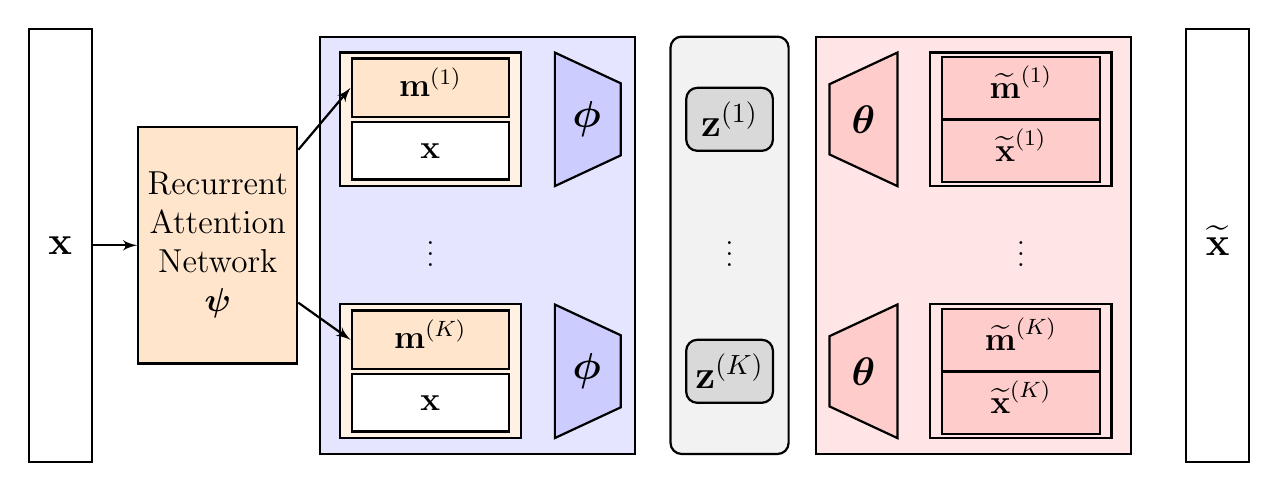
\begin{tikzpicture}[>=latex',thick]
      \node (rect) at (0,0)
      [draw, thick, minimum width=0.8cm, minimum height=5.5cm, name=x]
      {\Large{$\textbf{x}$}};

      \node (rect) at (5.3, 0)
      [draw, thick, minimum width=4cm, minimum height=5.3cm,
      fill=blue!10] {};


      \node (rect) at (11.6, 0)
      [draw, thick, minimum width=4cm, minimum height=5.3cm,
      fill=red!10] {};

      % \node (rect) at (1,1)
      % [draw, thick, minimum width=0.8cm, minimum height=2cm] {\Large{$\{\tbf{m}\}$}};

      \node (rect) at (2, 0)
      [draw, thick, minimum height=3cm, name=attention, fill=orange!20]
      {\large{\makecell[c]{Recurrent\\Attention\\Network\\$\boldsymbol{\psi}$}}};

      \draw [->] (x) -- (attention);

      \node (rect) at (4.7, 1.6)
      [draw, thick, minimum width=2.3cm, minimum height=1.7cm,
        fill=orange!10] {};

      \node (rect) at (4.7, 2)
      [draw, thick, minimum width=2cm, minimum height=0.7cm,
        name=attention, fill=orange!20, name=m1]
      {\large{\makecell[c]{$\textbf{m}^{(1)}$}}};
      \node (rect) at (4.7, 1.2)
      [draw, thick, minimum width=2cm, minimum height=0.7cm,
        name=attention, name=x1, fill=white]
      {\large{\makecell[c]{$\textbf{x}$}}};

      \draw [->] (attention) -- (m1.west);

      \node at (4.7, 0) {$\vdots$};


      \node (rect) at (4.7, -1.6)
      [draw, thick, minimum width=2.3cm, minimum height=1.7cm,
        fill=orange!10] {};

      \node (rect) at (4.7, -1.2)
      [draw, thick, minimum width=2cm, minimum height=0.7cm,
        name=attention, fill=orange!20, name=mK]
      {\large{\makecell[c]{$\textbf{m}^{(K)}$}}};

      \node (rect) at (4.7, -2)
      [draw, thick, minimum width=2cm, minimum height=0.7cm,
        name=attention, name=xK, fill=white]
      {\large{\makecell[c]{$\textbf{x}$}}};

      \draw [->] (attention) -- (mK.west);



      \node [trapezium, trapezium angle=65, minimum width=1.7cm,
        inner xsep=0.1cm, draw, thick, rotate=-90, fill=blue!20] at (6.7, 1.6)
      {\rotatebox{-90}{\Large{$\boldsymbol{\phi}$}}};

      \node [trapezium, trapezium angle=65, minimum width=1.7cm,
        inner xsep=0.1cm, draw, thick, rotate=-90, fill=blue!20] at (6.7, -1.6)
      {\rotatebox{-90}{\Large{$\boldsymbol{\phi}$}}};

      \node [rectangle, rounded corners] at (8.5, 0)
      [draw, thick, minimum width=1.5cm, minimum height=5.3cm,
      fill=gray!10] {};

      \node [rectangle, rounded corners]
      at (8.5, 1.6) [draw, thick, minimum width=1.1cm, minimum height=0.8cm,
      fill=gray!30] {\Large{$\textbf{z}^{(1)}$}};


      \node at (8.5, 0) {$\vdots$};

      \node [rectangle, rounded corners]
        at (8.5, -1.6) [draw, thick, minimum width=1.1cm, minimum height=0.8cm,
        fill=gray!30] {\Large{$\textbf{z}^{(K)}$}};

      \node [trapezium, trapezium angle=65, minimum width=1.7cm, inner xsep=0.1cm,
        draw, thick, rotate=90, fill=red!20] at (10.2, 1.6)
      {\rotatebox{-90}{\Large{$\boldsymbol{\theta}$}}};

      \node [trapezium, trapezium angle=65, minimum width=1.7cm, inner xsep=0.1cm,
        draw, thick, rotate=90, fill=red!20] at (10.2, -1.6)
      {\rotatebox{-90}{\Large{$\boldsymbol{\theta}$}}};


      \node (rect) at (12.2, 1.6)
      [draw, thick, minimum width=2.3cm, minimum height=1.7cm,
        fill=red!10] {};

      \node (rect) at (12.2, 2)
      [draw, thick, minimum width=2cm, minimum height=0.7cm,
        name=attention, fill=red!20, name=mK]
      {\large{\makecell[c]{$\widetilde{\textbf{m}}^{(1)}$}}};

      \node (rect) at (12.2, 1.2)
      [draw, thick, minimum width=2cm, minimum height=0.7cm,
        name=attention, name=xK, fill=red!20]
      {\large{\makecell[c]{$\widetilde{\textbf{x}}^{(1)}$}}};

      \node (rect) at (12.2, -1.6)
      [draw, thick, minimum width=2.3cm, minimum height=1.7cm,
        fill=red!10] {};

      \node (rect) at (12.2, -1.2)
      [draw, thick, minimum width=2cm, minimum height=0.7cm,
        name=attention, fill=red!20, name=mK]
      {\large{\makecell[c]{$\widetilde{\textbf{m}}^{(K)}$}}};

      \node (rect) at (12.2, -2)
      [draw, thick, minimum width=2cm, minimum height=0.7cm,
        name=attention, name=xK, fill=red!20]
      {\large{\makecell[c]{$\widetilde{\textbf{x}}^{(K)}$}}};


      \node at (12.2, 0) {$\vdots$};

      \node (rect) at (14.7,0)
      [draw, thick, minimum width=0.8cm, minimum height=5.5cm]
      {\makecell[c]{\Large{$\widetilde{\textbf{x}}$}}};

      % \node at (13.3, 2.3) {$\sum_k \textbf{m}_k \odot \widetilde{\textbf{x}}_k$};
    \end{tikzpicture}
\end{document}
